\subsection{Resultados da Simulação}
\label{subsec:resultadoSimulacao}

	Diversas simulações foram realizadas no simulador GRUBiX, como descrito na Seção \ref{subsec:simulacao}. As simulações foram realizadas para avaliar o comportamento do agente em redes com diferentes níveis de densidade de nós e distância de comunicação dos nós. Também foram simuladas redes somente com veículos sem uma infraestrutura de apoio e outra híbrida.

	Após realizar as simulações, os dados foram organizados e analisados em três fases:

	\begin{enumerate}
		\item Resultados obtidos na rede sem infraestrutura.
		\item Resultados obtidos na rede híbrida.
		\item Comparação dos resultados obtidos nas duas situações.
	\end{enumerate} 

	\subsubsection{Rede sem infraestrutura}
	\label{subsubsection:redeSemInfraestruturaResultadoDiscucao}

	Os resultados obtidos da rede sem infraestrutura mostram que o raio de alcance e a quantidade dos nós afetam o desempenho do agente. A Figura \ref{fig:graficosSemTorres} demonstra a evolução do tempo que o agente permaneceu na região alvo (desempenho do agente) com o aumento do raio e a quantidade de nós. 

	\begin{figure}[htbp]
		\centering
		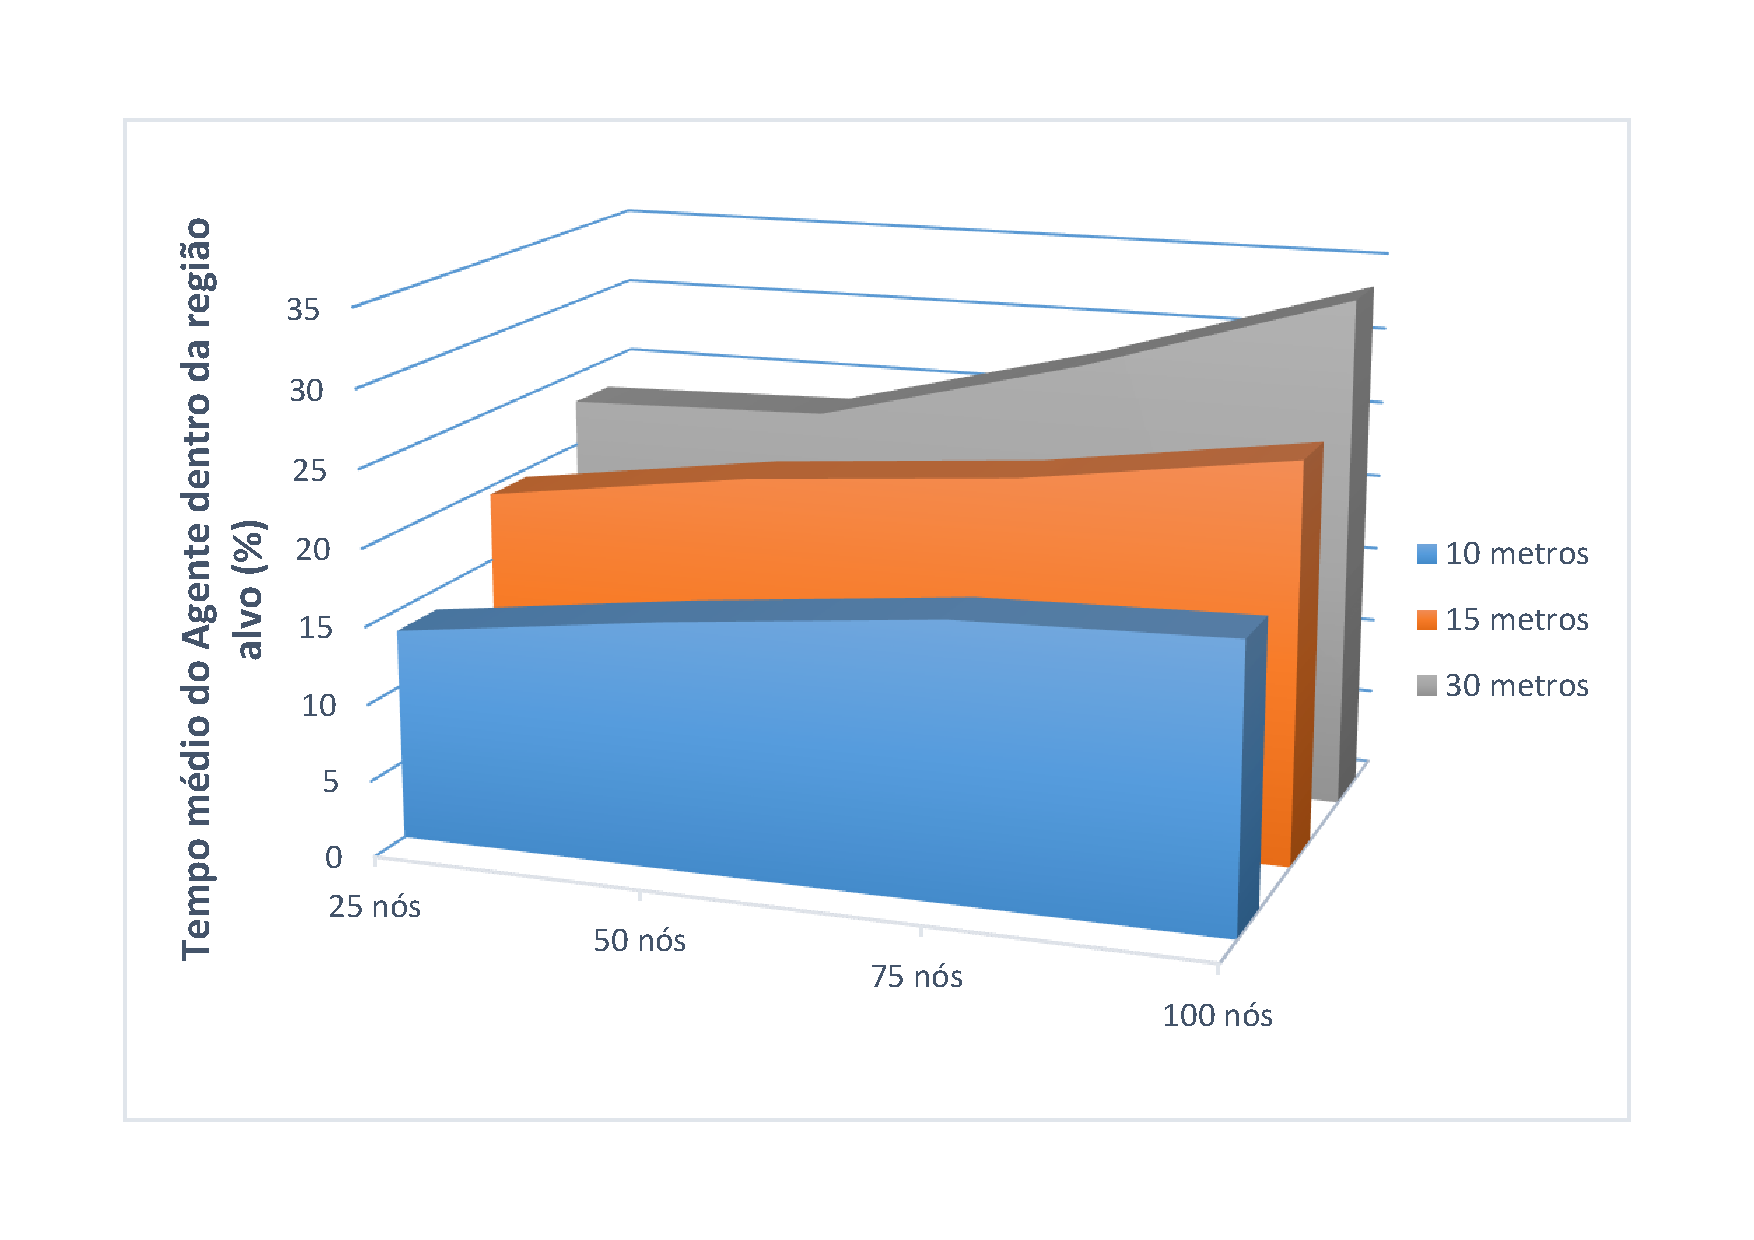
\includegraphics[scale=0.34]{resultados/graficos/graficoSemTorres.pdf}
		\caption{Resultados obtidos nos cenários sem infraestrutura.}
		\label{fig:graficosSemTorres}
	\end{figure}

	Na Tabela \ref{tab:estatiscaResultadosObtidosSemInfraestrutura} é possível visualizar a média aritmética, o desvio padrão e a variância dos resultados obtidos. 

	\begin{table}[!htb]
	    \caption{Estátistica dos resultados obtidos relativos a situação sem infraestrutura.}
	    \label{tab:estatiscaResultadosObtidosSemInfraestrutura}
	    \centering
	    \tiny
	    \begin{minipage}{.5\linewidth}
	      
	      \centering
	        \begin{tabular}{|c|c|c|c|}

			\hline
			\multicolumn{4}{|c|}{25 nós} \\ \hline
			Alcance   & média aritmética &	Desvio Padrão &	Variância  \\ \hline
			10 metros &	13,67 & 2,25 &	5,27  \\ \hline
			15 metros &	19,45 & 1,71 &	3,31  \\ \hline
			30 metros &	23,03 & 0,81 &	1,19 \\ \hline

			\multicolumn{4}{|c|}{} \\ \hline

			\multicolumn{4}{|c|}{50 nós} \\ \hline
			Alcance   & média aritmética &	Desvio Padrão &	Variância  \\ \hline
			10 metros &	15,96	& 1,41 & 2,25  \\ \hline
			15 metros &	21,95	& 1,43 & 2,52  \\ \hline
			30 metros &	23,48	& 1,12 & 1,80 \\ \hline

		\end{tabular}
	    \end{minipage}%
	    \begin{minipage}{.5\linewidth}
	      \centering
	        \begin{tabular}{|c|c|c|c|}
	        \hline
			\multicolumn{4}{|c|}{75 nós} \\ \hline
			Alcance   & média aritmética &	Desvio Padrão &	Variância  \\ \hline
			10 metros &	17,84 & 2,63 & 7,25  \\ \hline
			15 metros &	23,44 & 2,33 & 5,97  \\ \hline
			30 metros &	28,01 & 1,41 & 2,78 \\ \hline

			\multicolumn{4}{|c|}{} \\ \hline


			\multicolumn{4}{|c|}{100 nós} \\ \hline
			Alcance   & média aritmética &	Desvio Padrão &	Variância  \\ \hline
			10 metros &	18,40	& 2,86 & 8,52  \\ \hline
			15 metros &	26,01	& 1,40 & 2,65  \\ \hline
			30 metros &	33,48	& 1,10 & 2,33 \\ \hline

		\end{tabular}

	    \end{minipage} 
	\end{table}

Conforme o gráfico, a cada vinte e cinco nós que são adicionados a rede, a eficiência do agente aumenta. Quando o aumento ocorre no raio do alcance do nó, a melhora do desempenho também é perceptível. 

O aumento da eficiência do nó quando comparando o aumento do alcance de 10 metros para 15 metros foi maior que o aumento do alcance de 15 metros para 30 metros. Isso ocorre porque com o aumento do raio somente uma pequena parte do aumento da área coberta fica sobre a rua onde estão os veículos. A Figura \ref{fig:problemaDisperdicio} demonstra o problema. A região cinza representa as quadras e a região vermelha é a representação do sinal desperdiçado. Quanto maior o raio de alcance do nó, maior o desperdício. Essa é uma desvantagem em não usar rede híbrida porque dentro das quadras poderiam haver outros dispositivos que auxiliariam o agente. Assim o agente poderia encontrar rotas através das quadras, aumentando a quantidade de rotas disponíveis para ele usar.%Isso é algo que foi notado no experimento procurando referencia. 

\begin{figure}[htbp]
		\centering
		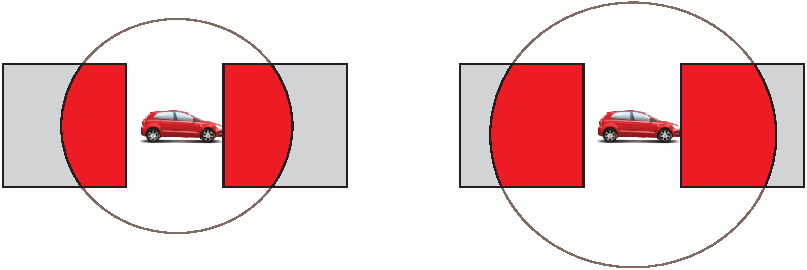
\includegraphics[scale=0.5]{resultados/figuras/problemaDisperdicio.pdf}
		\caption{Exemplificação do disperdicio.}
		\label{fig:problemaDisperdicio}
	\end{figure}


A princípio, não é necessário se preocupar com a economia de energia do transmissor/receptor instalado em cada veículo. Assim, o alcance da comunicação dos nós pode ser alta, melhorando o desempenho do agente. 

Quanto maior é a quantidade de veículos (nós) que formam a rede, maior é a probabilidade do agente alcançar novos nós hospedeiros, e assim maiores são as chances dele conseguir se manter na região alvo. A melhora de desempenho do agente comparando entre a situação onde o agente tem a disposição o menor alcance e a menor densidade de veículos (25 nós e 10 metros) para a situação mais farta de recursos (100 nós e 30 metros) é de 145\% aproximadamente.   


\subsubsection{Rede com infraestrutura}

	Os resultados obtidos em uma rede veicular com infraestrutura demonstrou que a densidade e raio de alcance tem os mesmos impactos discutidos na Seção \ref{subsubsection:redeSemInfraestruturaResultadoDiscucao}.

	Na Figura \ref{fig:graficosComTorres} demonstra a melhoria de desempenho do agente ao aumentar a densidade dos nós e o raio de alcance. A melhoria de desempenho do agente na configuração com a menor quantidade de recursos para a rede com a configuração com maior quantidade de recursos foi de 114,43\%.   
 

	\begin{figure}[htbp]
		\centering
		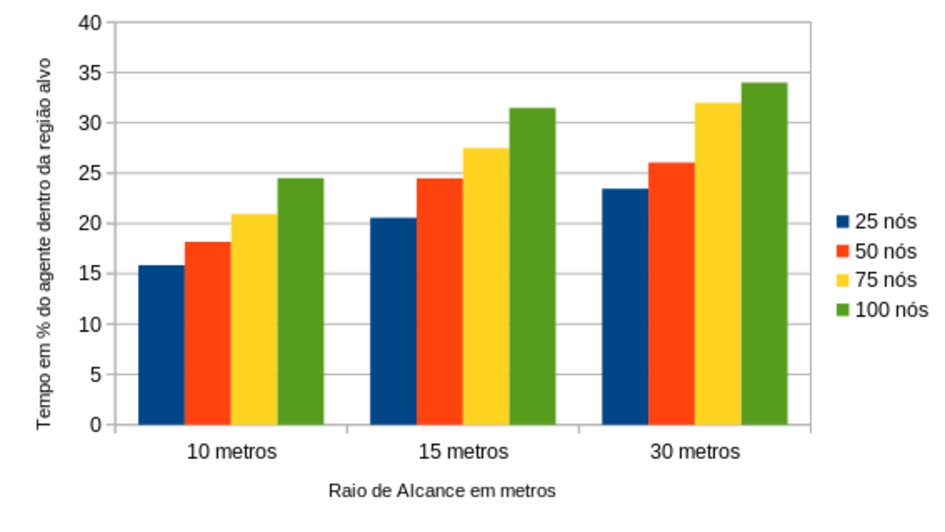
\includegraphics[scale=0.34]{resultados/graficos/graficoComTorres.pdf}
		\caption{Resultados obtidos no cenários com infraestrutura.}
		\label{fig:graficosComTorres}
	\end{figure}

	Para cada vinte e cinco nós que entram na rede, o agente melhora o seu desempenho (tempo médio dentro da região alvo) significativamente. O aumento do raio de alcance de cada nó também aumenta o desempenho do agente. O aumento combinado do raio e a densidade causa um impacto diretamente na quantidade de veículos que o agente tem acesso, aumentando o seu desempenho.

	Na Tabela \ref{tab:estatiscaResultadosObtidosComInfraestrutura} é possível visualizar a média aritmética, o desvio padrão e a variância dos resultados obtidos.

	\begin{table}[!htb]
	    \caption{Estatística dos resultados obtidos}
	    \label{tab:estatiscaResultadosObtidosComInfraestrutura}
	    \centering
	    \tiny
	    \begin{minipage}{.5\linewidth}
	      
	      \centering
	        \begin{tabular}{|c|c|c|}

			\hline
			\multicolumn{3}{|c|}{25 nós} \\ \hline
			Alcance   & média aritmética &	Desvio Padrão   \\ \hline
			10 metros &	15,85 & 1,40   \\ \hline
			15 metros &	20,57 & 1,68   \\ \hline
			30 metros &	23,45 & 1,11  \\ \hline

			\multicolumn{3}{|c|}{} \\ \hline

			\multicolumn{3}{|c|}{50 nós} \\ \hline
			Alcance   & média aritmética &	Desvio Padrão   \\ \hline
			10 metros &	18,18 & 1,43   \\ \hline
			15 metros &	24,48 & 1,12  \\ \hline
			30 metros &	26,05 & 1,41  \\ \hline

		\end{tabular}
	    \end{minipage}%
	    \begin{minipage}{.5\linewidth}
	      \centering
	        \begin{tabular}{|c|c|c|}
	        \hline
			\multicolumn{3}{|c|}{75 nós} \\ \hline
			Alcance   & média aritmética &	Desvio Padrão   \\ \hline
			10 metros &	20,94 & 2,05   \\ \hline
			15 metros &	27,50 & 1,69   \\ \hline
			30 metros &	31,99 & 1,38 \\ \hline

			\multicolumn{3}{|c|}{} \\ \hline


			\multicolumn{3}{|c|}{100 nós} \\ \hline
			Alcance   & média aritmética &	Desvio Padrão   \\ \hline
			10 metros &	24,51 & 1,10   \\ \hline
			15 metros &	31,49 & 1,13   \\ \hline
			30 metros &	34,00 & 1,42  \\ \hline

		\end{tabular}

	    \end{minipage} 
	\end{table}  


\subsubsection{Comparando Redes com infraestrutura e Redes sem infraestrutura}

Comparando o aumento da quantidade dos nós o agente permaneceu na região alvo em média um período 12,95\% maior na redes com infraestrutura. A Figura \ref{fig:comparacaoVariacaoNos} é foi obtida através das médias dos alcance dos nós. Com isso pode-se comparar o impacto da variação da quantidade de nós no desempenho do agente nos dois tipos de redes. 

\begin{figure}[htbp]
	\centering
	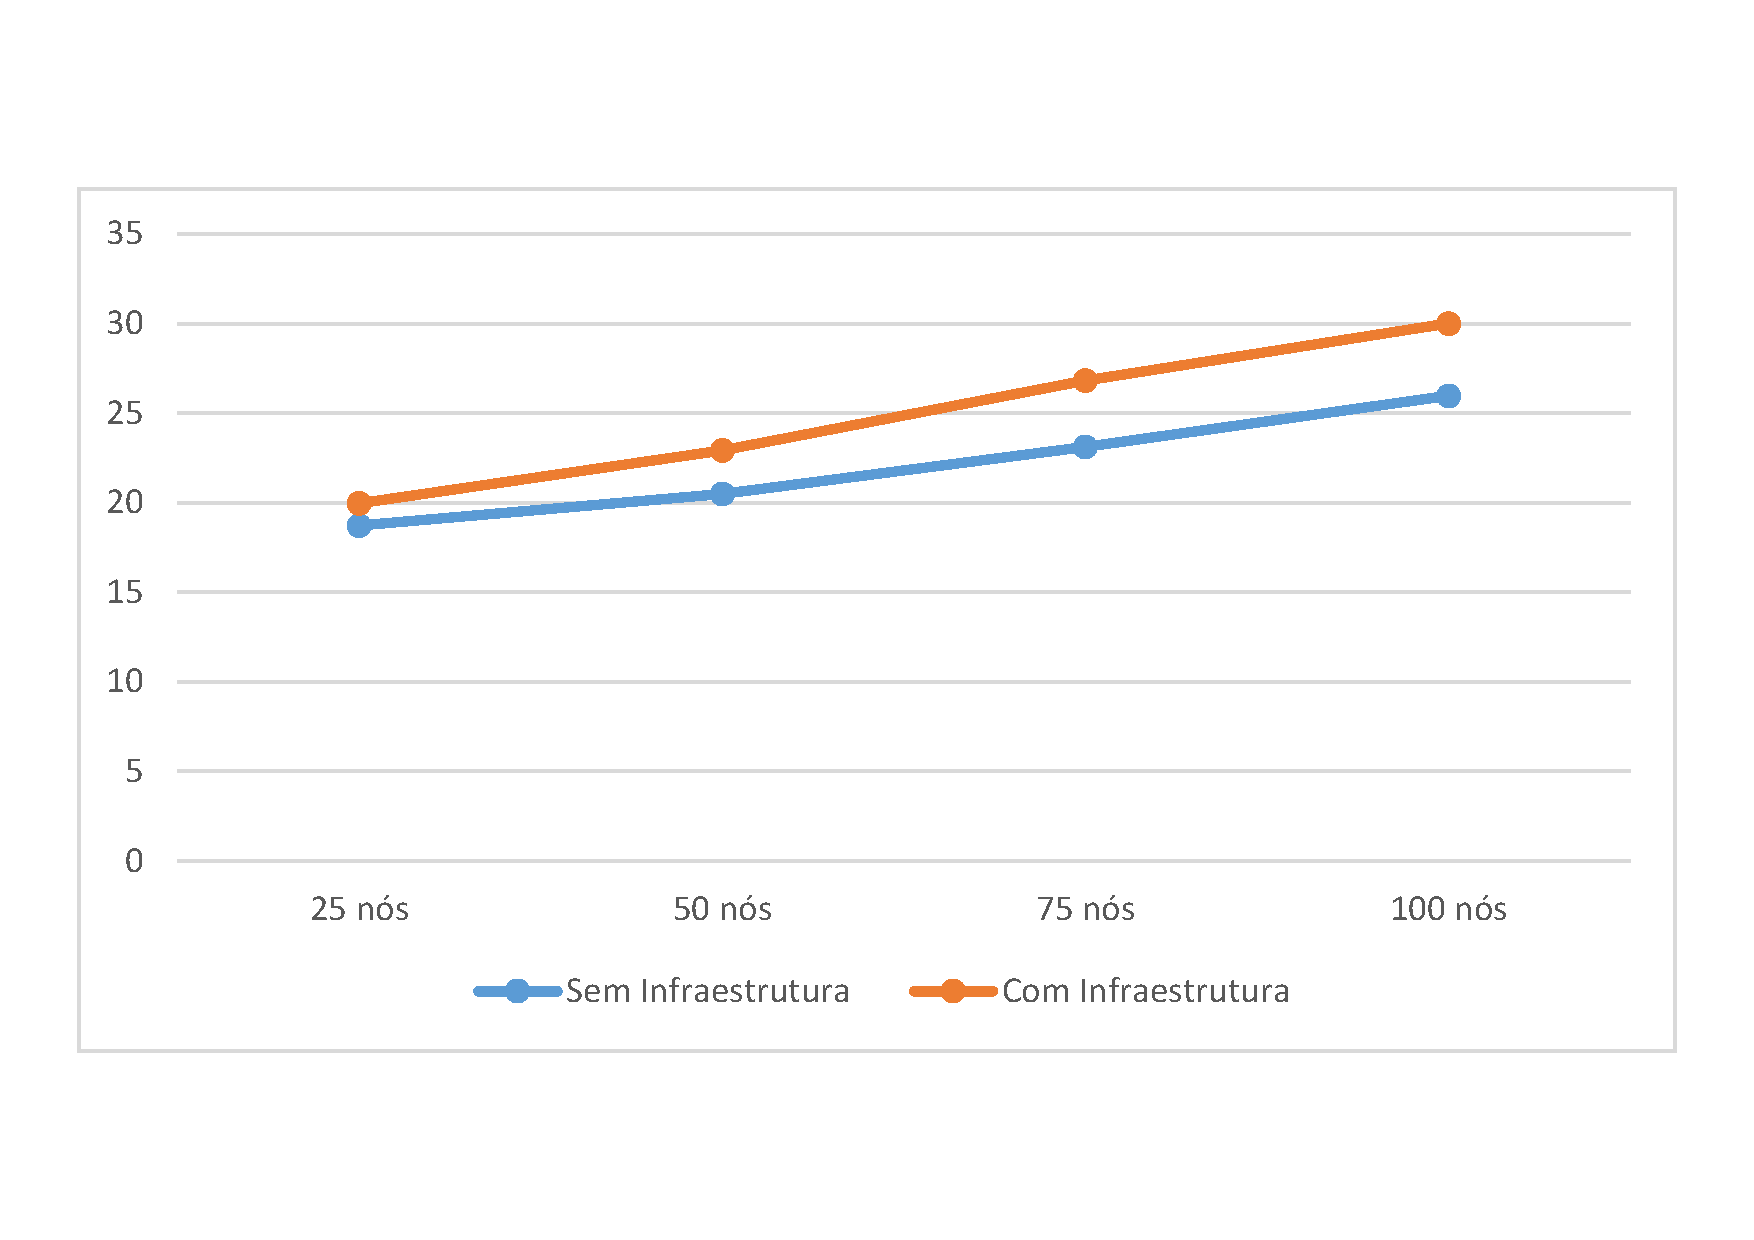
\includegraphics[scale=0.34]{resultados/graficos/comparacaoVariacaoNos.pdf}
	\caption{Comparação do impacto da variação da quantidade de nós nos dois tipos de redes}
	\label{fig:comparacaoVariacaoNos}
\end{figure}  


Para avaliar o impacto do raio de alcance do nó foi realizado a média do tempo que o agente permaneceu na região alvo nas diferentes configurações de densidade. Com o aumento do raio o agente permanceu na ragião alvo um tempo médio 12,95\% maior. A Figura \ref{fig:comparacaoVariacaoRaioAlcance} demonstra a comparação do tempo médio que o agente permaneceu na região alvo em relação ao raio de alcance.

\begin{figure}[htbp]
	\centering
	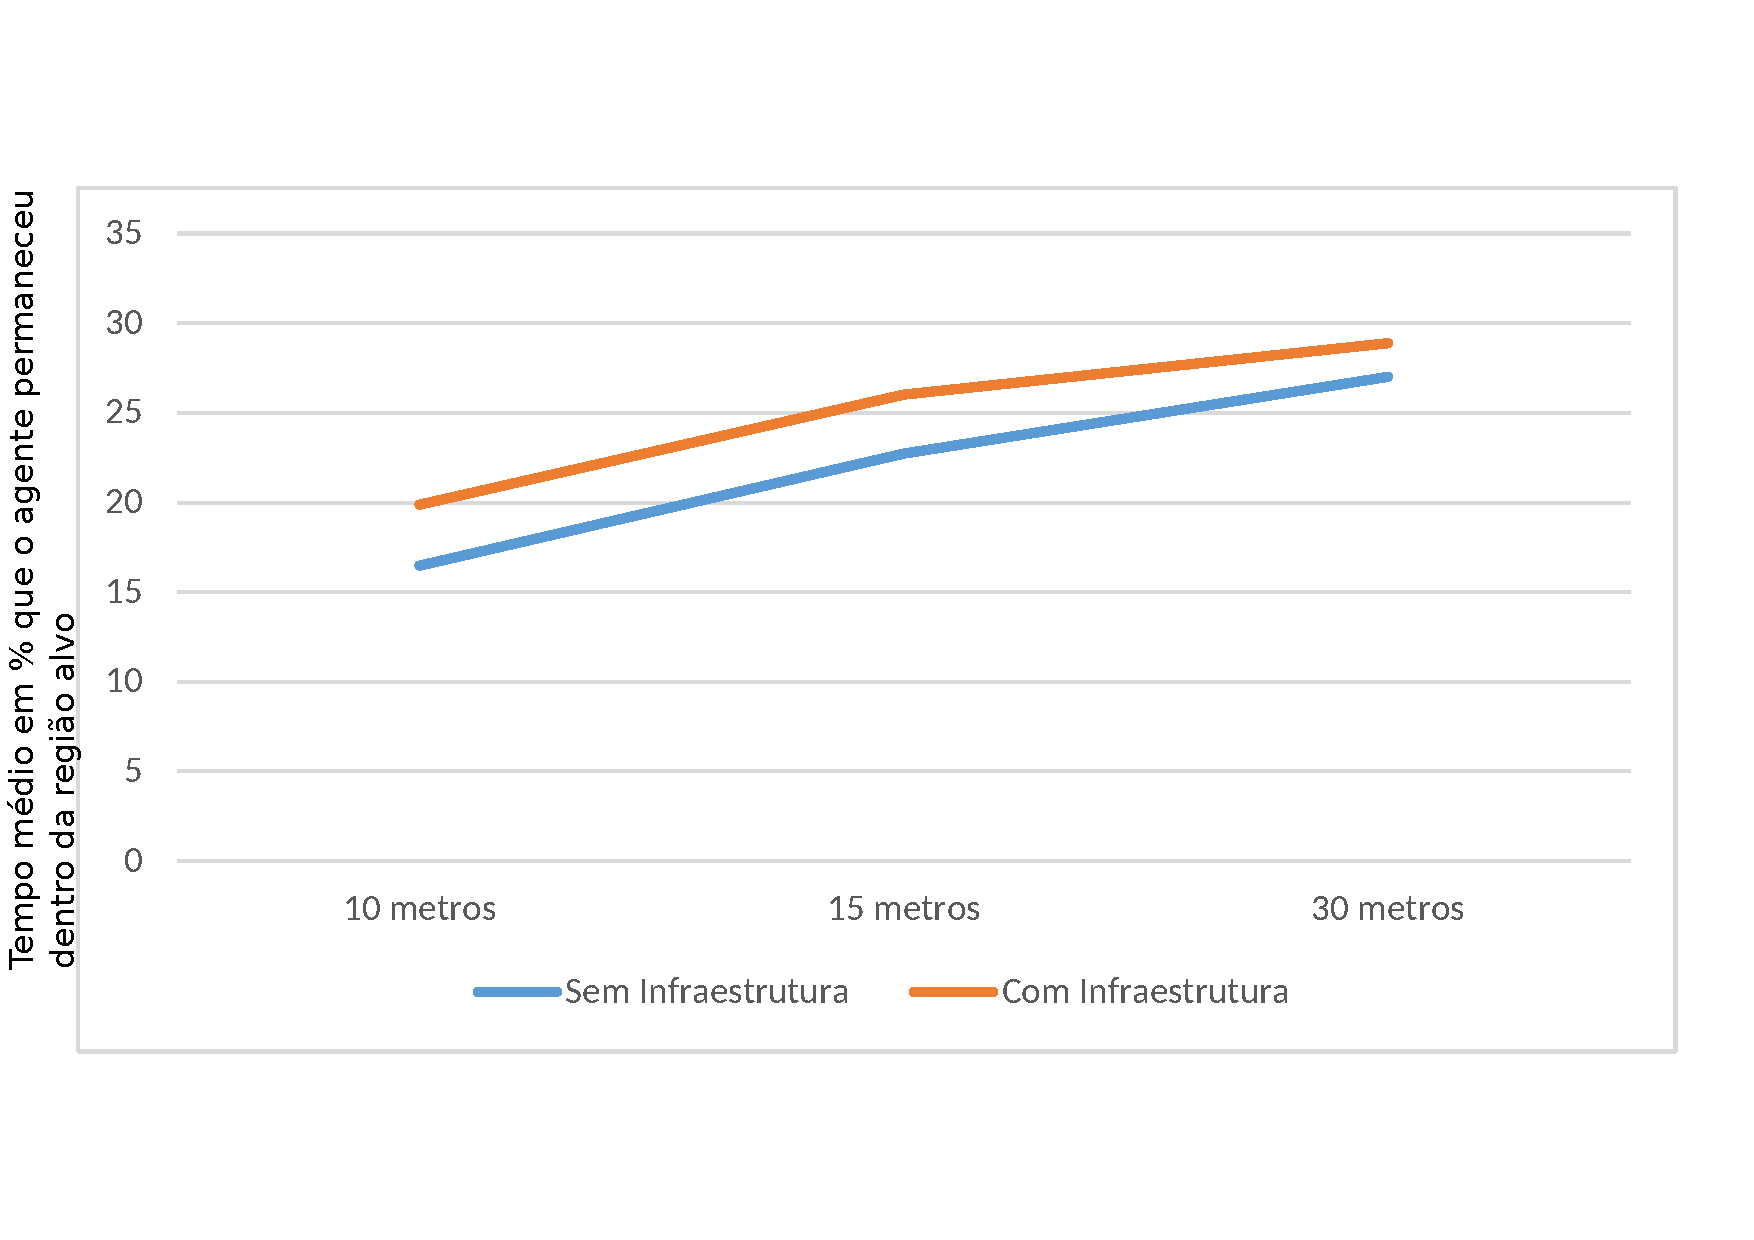
\includegraphics[scale=0.34]{resultados/graficos/comparacaoVariacaoRaioAlcance.pdf}
	\caption{Comparação do impacto da variação do raio de alcance nos dois tipos de redes.}
	\label{fig:comparacaoVariacaoRaioAlcance}
\end{figure}

Na Figura \ref{fig:comparacaoMelhoriaComVariacaoRaioAlcance} pode-se observar um comportamento semelhante ao caso do aumento de nós. Com o aumento do raio de alcance do nó, aumenta a quantidade de veículos que o agente pode escolher como hospedeiro. Assim o agente tem mais chances de encontrar um veículo que passe na região alvo. Quanto maior o raio de alcance do nó, menor é o impacto da infraestrutura em relação a rede sem ela.

\begin{figure}[htbp]
	\centering
	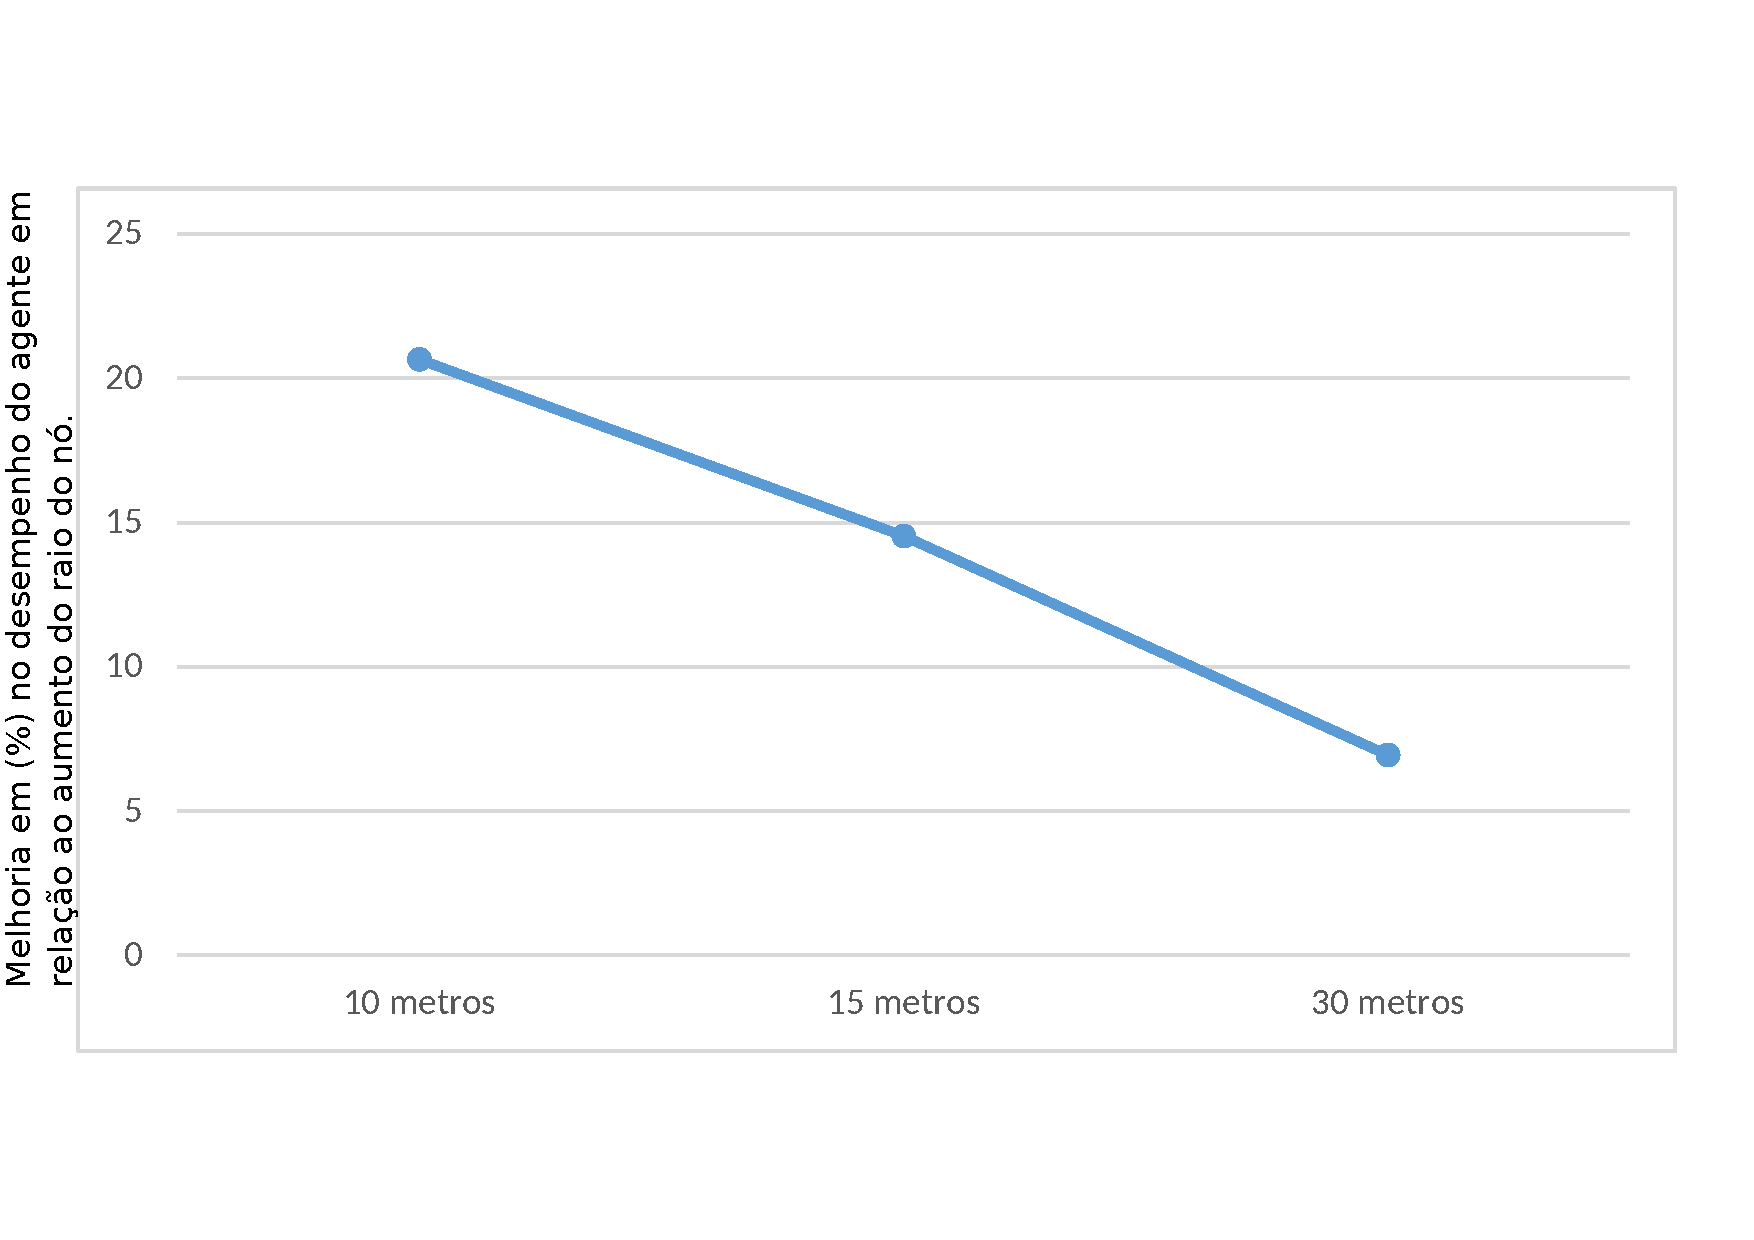
\includegraphics[scale=0.34]{resultados/graficos/comparacaoMelhoriaComVariacaoRaioAlcance.pdf}
	\caption{Melhoria da rede com infraestrutura em relação a rede sem infraestrutura com o aumento da quantidade de nós.}
	\label{fig:comparacaoMelhoriaComVariacaoRaioAlcance}
\end{figure}

Observando os dois resultados, a infraestrutura auxilia o agente em chegar a região alvo até um limite de veículos e raio de alcance. Porém, em redes onde a densidade é alta e o raio também, a infraestrutura não promove um grande aumento de desempenho.
